\documentclass[review]{elsarticle}

\usepackage{amsmath}
\usepackage{booktabs}
\usepackage{dirtytalk}
\usepackage{subcaption}
\usepackage{tabularx}
\usepackage[usenames]{xcolor}
\usepackage{lineno,hyperref}
\modulolinenumbers[5]

\journal{Composites Part A}

%%%%%%%%%%%%%%%%%%%%%%%
%% Elsevier bibliography styles
%%%%%%%%%%%%%%%%%%%%%%%
%% To change the style, put a % in front of the second line of the current style and
%% remove the % from the second line of the style you would like to use.
%%%%%%%%%%%%%%%%%%%%%%%

%% Numbered
%\bibliographystyle{model1-num-names}

%% Numbered without titles
%\bibliographystyle{model1a-num-names}

%% Harvard
%\bibliographystyle{model2-names.bst}\biboptions{authoryear}

%% Vancouver numbered
%\usepackage{numcompress}\bibliographystyle{model3-num-names}

%% Vancouver name/year
%\usepackage{numcompress}\bibliographystyle{model4-names}\biboptions{authoryear}

%% APA style
%\bibliographystyle{model5-names}\biboptions{authoryear}

%% AMA style
%\usepackage{numcompress}\bibliographystyle{model6-num-names}

%% `Elsevier LaTeX' style
\bibliographystyle{elsarticle-num}
%%%%%%%%%%%%%%%%%%%%%%%

\begin{document}

\begin{frontmatter}

\title{Energy release rate of the fiber/matrix interface crack growth in $\left[0_{m\cdot2l}^{\circ},90_{l}^{\circ}\right]_{S}$ laminates under transverse loading: effect of $0^{\circ}/90^{\circ}$ interface}
%\tnotetext[mytitlenote]{Fully documented templates are available in the elsarticle package on \href{http://www.ctan.org/tex-archive/macros/latex/contrib/elsarticle}{CTAN}.}

%% Group authors per affiliation:
%\author{Luca Di Stasio\fnref{myfootnote}}
%\address{Radarweg 29, Amsterdam}
%\fntext[myfootnote]{Since 1880.}

%% or include affiliations in footnotes:
\author[nancy,lulea]{Luca Di Stasio}
\author[lulea]{Janis Varna}
\author[nancy]{Zoubir Ayadi}
%\ead[url]{www.elsevier.com}

%\author[mysecondaryaddress]{Global Customer Service\corref{mycorrespondingauthor}}
%\cortext[mycorrespondingauthor]{Corresponding author}
%\ead{support@elsevier.com}

\address[nancy]{Universit\'e de Lorraine, EEIGM, IJL, 6 Rue Bastien Lepage, F-54010 Nancy, France}
\address[lulea]{Lule\aa\ University of Technology, University Campus, SE-97187 Lule\aa, Sweden}

\begin{abstract}
\noindent
%\textcolor{purple}{{\em Priority}: 1}\\
%\textcolor{purple}{{\em Target journal(s)}: Composites Part B: Engineering, Composites Part A: Applied Science and Manufacturing, Composite Structures, Journal of Composite Materials, Composite Communications}\\
Models of Representative Volume Elements (RVEs) of cross-ply $\left[0_{m\cdot2l}^{\circ},90_{l}^{\circ}\right]_{S}$ laminates with different geometric configurations and damage states are studied. Debond growth is characterized by the estimation of the Mode I and Mode II Energy Release Rate (ERR) using the Virtual Crack Closure Technique (VCCT) and the J-integral. It is found that the presence of the $0^{\circ}/90^{\circ}$ interface and the thickness of the $0^{\circ}$ layer have no effect, apart from laminates with \emph{ultra-thin} $90^{\circ}$ plies where it is however modest. With the exception of cross-ply laminates with an \emph{ultra-thin} $90^{\circ}$ ply, no difference is found in debond ERR between a UD composite and a cross-ply laminate.
\end{abstract}

\begin{keyword}
Polymer-matrix Composites (PMCs)\sep Thin-ply\sep Transverse Failure \sep Debonding \sep Finite Element Analysis (FEA)
\end{keyword}


\end{frontmatter}

\linenumbers

%%%%%%%%%%%%%%%%%%%%%%%%%%%%%%%%%%%%%%%%%%%%%%%%%%%%%%%%%%%%%%%%%%%
% 1. INTRODUCTION
%%%%%%%%%%%%%%%%%%%%%%%%%%%%%%%%%%%%%%%%%%%%%%%%%%%%%%%%%%%%%%%%%%%

\section{Introduction}

Since the development of the \emph{spread tow} technology or \say{FUKUI method}~\cite{Kawabe2008,Kawabe2008en}, significant efforts have been directed toward the characterization of \emph{thin-ply} laminates~\cite{Sasayama2003,Yamaguchi2005,Tsai2005,Sihn2007,Yokozeki2008,Yokozeki2010,Saito2012,Arteiro2013,Arteiro2014,Amacher2014,Guillamet2014,Huang2018,Cugnoni2018} and their application to mission-critical structures in the aerospace sector~\cite{Moon2011,Kim2017,Kopp2017,McCarville2018}.\\
At the lamina level, the use of \emph{thin-plies} leads to more regular and homogeneous microstructures~\cite{Saito2012,Amacher2014}. Measurement of ply level properties (tensile and compressive modulus, Poisson's ratio, ultimate tensile strength,tensile onset of damage, interlaminar shear strength) on UD specimens ($\left[0_{m}^{\circ}\right]$ and $\left[90_{m}^{\circ}\right]$) revealed no remarkable difference with average properties available in the literature for the same type of fiber, nor showed any particular dependence on the ply thickness~\cite{Amacher2014}. Only an increase of the ultimate compressive strength in the fiber direction was observed with very thin plies ($\sim4$ fiber diameters), although with very scattered values, which the authors claim to be due to the fiber arrangement's increased regularity which prevents the onset of fiber microbuckling~\cite{Amacher2014}. A number of researchers~\cite{Yamaguchi2005,Tsai2005,Sihn2007,Yokozeki2008} has reported improvements in fatigue life with the use of \emph{thin-plies}, which are explained as a consequence of delayed propagation of free edge delaminations and intralaminar cracks. Several researchers have in fact analyzed the beneficial effect of \emph{thin-plies} on damage development under static~\cite{Sasayama2003,Sihn2007,Yokozeki2008,Yokozeki2010,Saito2012,Arteiro2013,Arteiro2014,Amacher2014}, fatigue~\cite{Yamaguchi2005,Sihn2007,Yokozeki2008,Yokozeki2010,Amacher2014} and impact loadings~\cite{Sihn2007,Yokozeki2008,Yokozeki2010,Amacher2014}. It seems apparent that \emph{thin-ply} laminates possess an increased ability to delay, and in some cases even suppress, the onset and propagation of intralaminar cracks (or transverse or matrix or micro-cracks).\\
The first appearance of transverse cracks is known to be characterized by the occurrence of fiber/matrix interface cracks (also referred to as debonds), which grow along the fiber arc direction, then kink out of the interface and coalesce forming a transverse crack~\cite{Bailey1981}. Different approaches have been applied to model the initiation and growth of debonds. The Cohesive Zone Model (CZM) has been used to mimic the propagation of debonds along fiber interfaces; coupled with a failure criterion for the matrix, it has provided simulations of the growth of transverse cracks starting from a virgin material~\cite{Kushch2011,Canal2012,Bouhala2013,Herraez2015}. The main advantages of this approach are the possibility to observe the development of a simulated crack path and to record a load-displacement curve to compare with experimental measurement. However, various observations cast a doubt about the applicability of the CZM: the bi- (for 2D models) and tri- (in 3D) axiality of the matrix stress state in the inter-fiber region that is linked with a cavitation-like failure of the polymer~\cite{Asp1995}; the locality and mode dependency of the interface failure~\cite{Mantic2009}; the problematic use at the microscopic level of properties measured in UD specimens at the laminate level~\cite{Canal2012}. A second approach that obviates these drawbacks is the application of Linear Elastic Fracture Mechanics (LEFM) arguments to the study of debond growth. The analysis focuses on the evaluation of Mode I and Mode II Energy Release Rate (ERR) at the crack tip by means of the Virtual Crack Closure Technique (VCCT)~\cite{Krueger2004} or the J-Integral method~\cite{Rice1968}. The stress and strain field, required for the ERR computation, can be solved by application of different methodologies such as analytical solutions~\cite{Toya1974}, the Boundary Element Method (BEM)~\cite{Paris1996} or the Finite Element Method (FEM)~\cite{Zhuang2018}. The limitation of this approach is that it describes propagation of the debond, not its initiation. Finite fracture mechanics~\cite{MunozReja2016} is one way how to address the initiation problem. Different works have followed the LEFM approach and studied models of one or two fibers in an effectively infinite matrix~\cite{Correa2011,Correa2013,Correa2014,Sandino2016,Sandino2018} and of an hexagonal cluster of fibers in an effectively infinite homogenized UD composite~\cite{Varna2017,Zhuang2018}. The problem of debond growth along the fiber-matrix interface in a cross-ply laminate has been only addressed very recently in~\cite{Velasco2018,Paris2018}, where authors embed a single partially debonded fiber in an effectively infinite homogenized $90^{\circ}$ ply bounded by homogenized $0^{\circ}$ layers. Thus, the effect of debond-debond interaction and of the relative proximity of a $0^{\circ}/90^{\circ}$ interface on the debond's ERR in cross-ply laminates is yet to be addressed. The present work is devoted to this problem. Models of Repeating Unit Cells (RUCs) are developed to represent laminates with different degrees of damage (here only in the form of debonds). The number of fully bonded fibers across the thickness of the $90^{\circ}$ ply is varied in order to investigate the effect of the proximity of the $0^{\circ}/90^{\circ}$ interface. The thickness of the bounding $0^{\circ}$ layers is also used as a parameter of the study. The stress and strain fields are solved with the Finite Element Method in Abaqus~\cite{abq12} and the debond (crack) is characterized by its Mode I and Mode II ERR, calculated with the VCCT and the J-integral method.

%%%%%%%%%%%%%%%%%%%%%%%%%%%%%%%%%%%%%%%%%%%%%%%%%%%%%%%%%%%%%%%%%%%
% 2. RVE MODELS AND FE DISCRETIZATION
%%%%%%%%%%%%%%%%%%%%%%%%%%%%%%%%%%%%%%%%%%%%%%%%%%%%%%%%%%%%%%%%%%%

\section{RVE models \& FE discretization}

% 2.1 Introduction and nomenclature

\subsection{Introduction \& Nomenclature}\label{subsec:names}

In the present work, we investigate debond development under in-plane transverse tension in $\left[0_{m\cdot2l}^{\circ},90_{l}^{\circ}\right]_{S}$ laminates, where $2l$ is the thickness of the central $90^{\circ}$ layer expressed in terms of the number $l$ of plies constituting it and $m\cdot2l$ represents the thickness of the $0^{\circ}$ layer as a multiple of the $90^{\circ}$ layer thickness. The interaction between debonds in the presence of an interface with a stiff layer is studied with the use of different Repeating Unit Cells (RUCs)  (see Figures~\ref{fig:laminateModelsA} and~\ref{fig:laminateModelsB} in Sec.~\ref{subsec:rve}), in which only the central fiber is partially debonded. Repetition of the composite RUC can occur only along the in-plane transverse direction, thus representing a cross-ply laminate with a thin or even ultra-thin $90^{\circ}$ ply in the middle.\\
The thickness of the $90^{\circ}$ ply depends on the number of fibers present across the thickness (the vertical or $z$ direction in Figures~\ref{fig:laminateModelsA} and~\ref{fig:laminateModelsB}) and the value of the fiber volume fraction $V_{f}$. On the other hand, the thickness of the $0^{\circ}$ layers can be assigned freely as a multiple of the $90^{\circ}$ ply thickness, i.e. $t_{0^{\circ}}=m\cdot t_{90^{\circ}}$ where $m$ is an arbitrary integer. Thus, the thickness ratio $i$ represents one additional parameter for the investigation. In the RUCs proposed, we consider the $90^{\circ}$ ply with debonds as a series of stacked damaged and undamaged fiber rows, each row with only one fiber in the thickness direction. All the RUCs present regular microstructures with fibers placed according to a square-packing configuration and consequently they are Representative Volume Elements (RVE) of cross-ply laminates with a certain distribution of debonds in the middle $90^{\circ}$ layer. In the following, let us consider in-plane coordinates $x$ and $y$, where $x$ is in the transverse direction of the cross-ply laminate under consideration. In the presence of a load in the $x$-direction, the strain in the $y$-direction is small, due to the very small Poisson's ratio of the laminate. Furthermore, debonds are considered to be significantly longer in the fiber direction than in the arc direction~\cite{Zhang1997}. Therefore we use 2D models under the assumption of plane strain, defined in the $x-z$ section of the composite. The study presented in this paper thus applies to long debonds and its focus ia on understanding the mechanisms of growth along their arc direction. The laminates are assumed to be subject to transverse tensile strain, which is applied in the form of a constant displacement in the $x$-direction along both vertical boundaries of the RUC as shown in  Figure~\ref{fig:modelschem}.\\
In summary, the models are differentiated by: first, the spacing between debonds along the horizontal direction in the $90^{\circ}$ layer, which corresponds to the number $n$ of fibers in the RUC's horizontal direction; second, the thickness of the middle $90^{\circ}$ ply measured in terms of the number $k$ of fiber rows; third, the factor $m$ which provides the thickness of the $0^{\circ}$ layers as an integer multiple of the $90^{\circ}$ ply thickness.  It thus seems natural to introduce a common notation in the presented results as $n\times k-m\cdot t_{90^{\circ}}$. An additional model is considered to study the effect of equivalent boundary conditions. This final model is constituted by only one partially debonded fiber. The application of coupling of horizontal displacements in the form of a constant applied displacement along the right and left sides allows for repetition along the horizontal direction. The presence of coupling of vertical displacements and a linear distribution of horizontal displacements on the bottom and top surfaces models the presence of the interface between the $90^{\circ}$ layer and the stiff $0^{\circ}$ one. This model is refered to as $1\times 1-H+V$ given that: it has respectively 1 fiber in the horizontal and in the vertical direction; on the top and bottom surfaces, both horizontal (H) and vertical (V) displacements are assigned. Furthermore, two single fiber models similar to  $1\times 1-H+V$ are considered in the present work for comparison: the  $1\times 1-free$ and  $1\times 1-coupling$. In the first, the upper surface is left free; in the second, vertical displacement coupling is applied to the upper boundary. Further details about these models and the corresponding laminate RVE can be found in~\cite{DiStasio2019}.

%% 2.2 Models of Representative Volume Element (RVE)

\subsection{Description of modelled Representative Volume Elements (RVEs)}\label{subsec:rve}

The first family of Representative Volume Elements (RVEs) is represented in Figure~\ref{fig:laminateModelsA}. It represents a set of $\left[0_{m\cdot2l}^{\circ},90_{l}^{\circ}\right]_{S}$ cross-ply laminates with an ultra-thin $90^{\circ}$ layer, constituted by a single row of fibers across the thickness. Debonds appear at regular intervals measured in terms of number $n-1$ of fully bonded fibers present between them, which in turn correspond to the number of fibers along the horizontal direction of the RVE as highlighted in Fig.~\ref{fig:laminateModelsA}. They are thus the $n\times1-m\cdot t_{90^{\circ}}$ models, where $m=1,10$ and $n$ is an integer $\geq1$ ($n=1$ corresponds to the case of a debond appearing on all the fibers in the central $90^{\circ}$ layer). These models are geometrically extreme, but allow to focus on the interaction between debonds and the inter-ply $0^{\circ}/90^{\circ}$ interface. Furthermore, the \emph{spread tow} technology is today capable of producing cross-ply laminates with the central $90^{\circ}$ layer thickness only $4-5$ times the fiber diameter, as shown for example in~\cite{Saito2012}, which may in future give practical relevance even to such extreme case.

\begin{figure}[!h]
\centering
  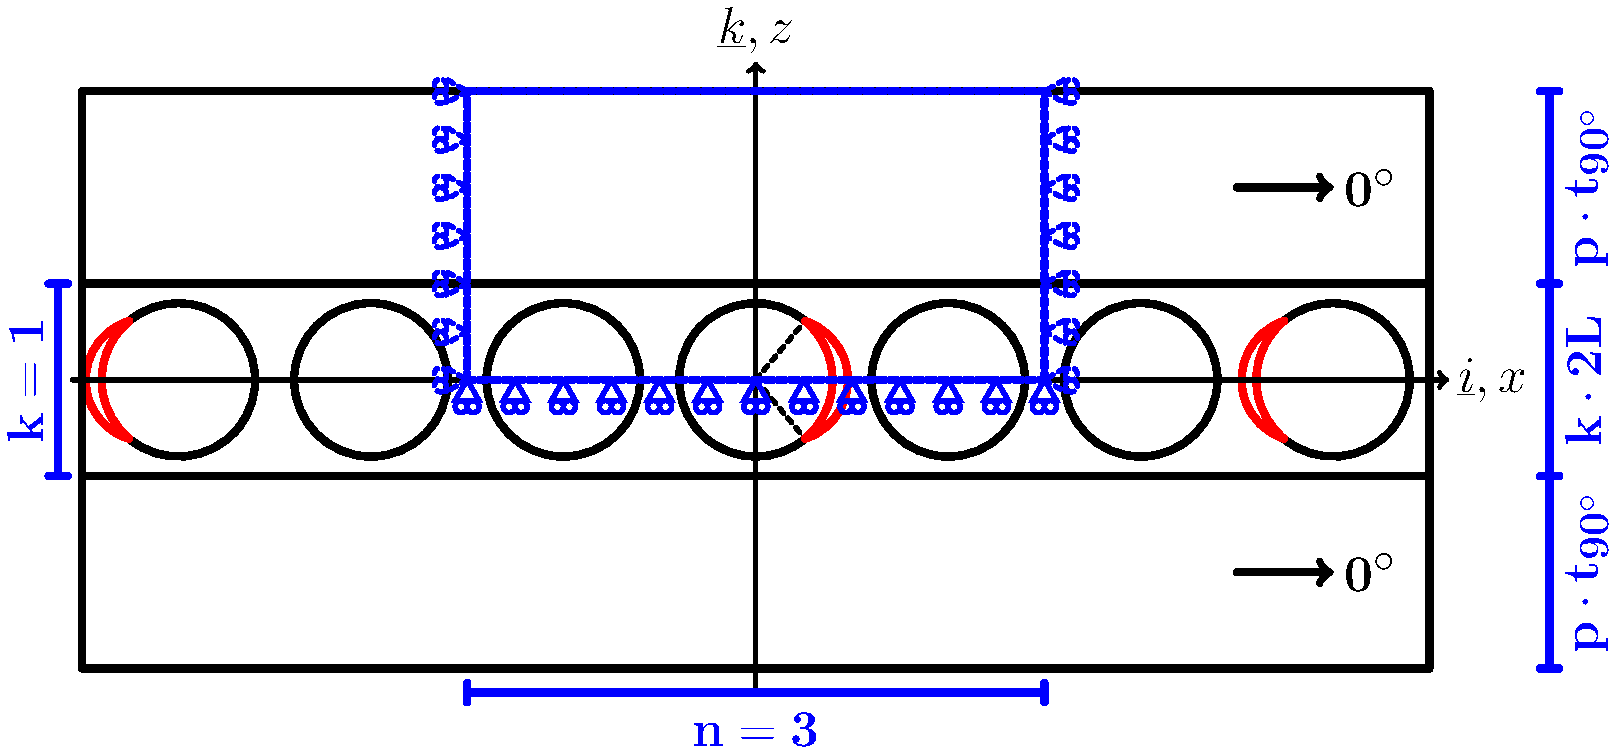
\includegraphics[width=\textwidth]{thinPly.pdf}
\caption{Models of $\left[0_{m\cdot2l}^{\circ},90_{l}^{\circ}\right]_{S}$ laminates with an ultra-thin $90^{\circ}$ layer, where the $90^{\circ}$ ply is made up by a single ``row'' of fibers. Debonds are repeating at different distances, measured in terms of the number $n-1$ of fully bonded fibers appearing between two consecutive debonds.}\label{fig:laminateModelsA}
\end{figure}

The second set of models considers instead cross-ply laminates with a central $90^{\circ}$ ply of variable thickness, measured in terms of number $k$ of fiber rows appearing in the vertical direction in Figure~\ref{fig:laminateModelsB}. Once again, debonds appear in the central row only at regular intervals measured in terms of number $n-1$ of fully bonded fibers present between them, which in turn correspond to the number of fibers along the horizontal direction of the RUC as highlighted in Fig.~\ref{fig:laminateModelsB}. These models are thus the $n\times k-m\cdot t_{90^{\circ}}$ models, where $i=1,10$, $k>1$ and $n$ is an integer $\geq1$ ($n=1$ corresponds to the case of a debond appearing on all fibers of the central fiber row in the $90^{\circ}$ layer).

\begin{figure}[!h]
\centering
        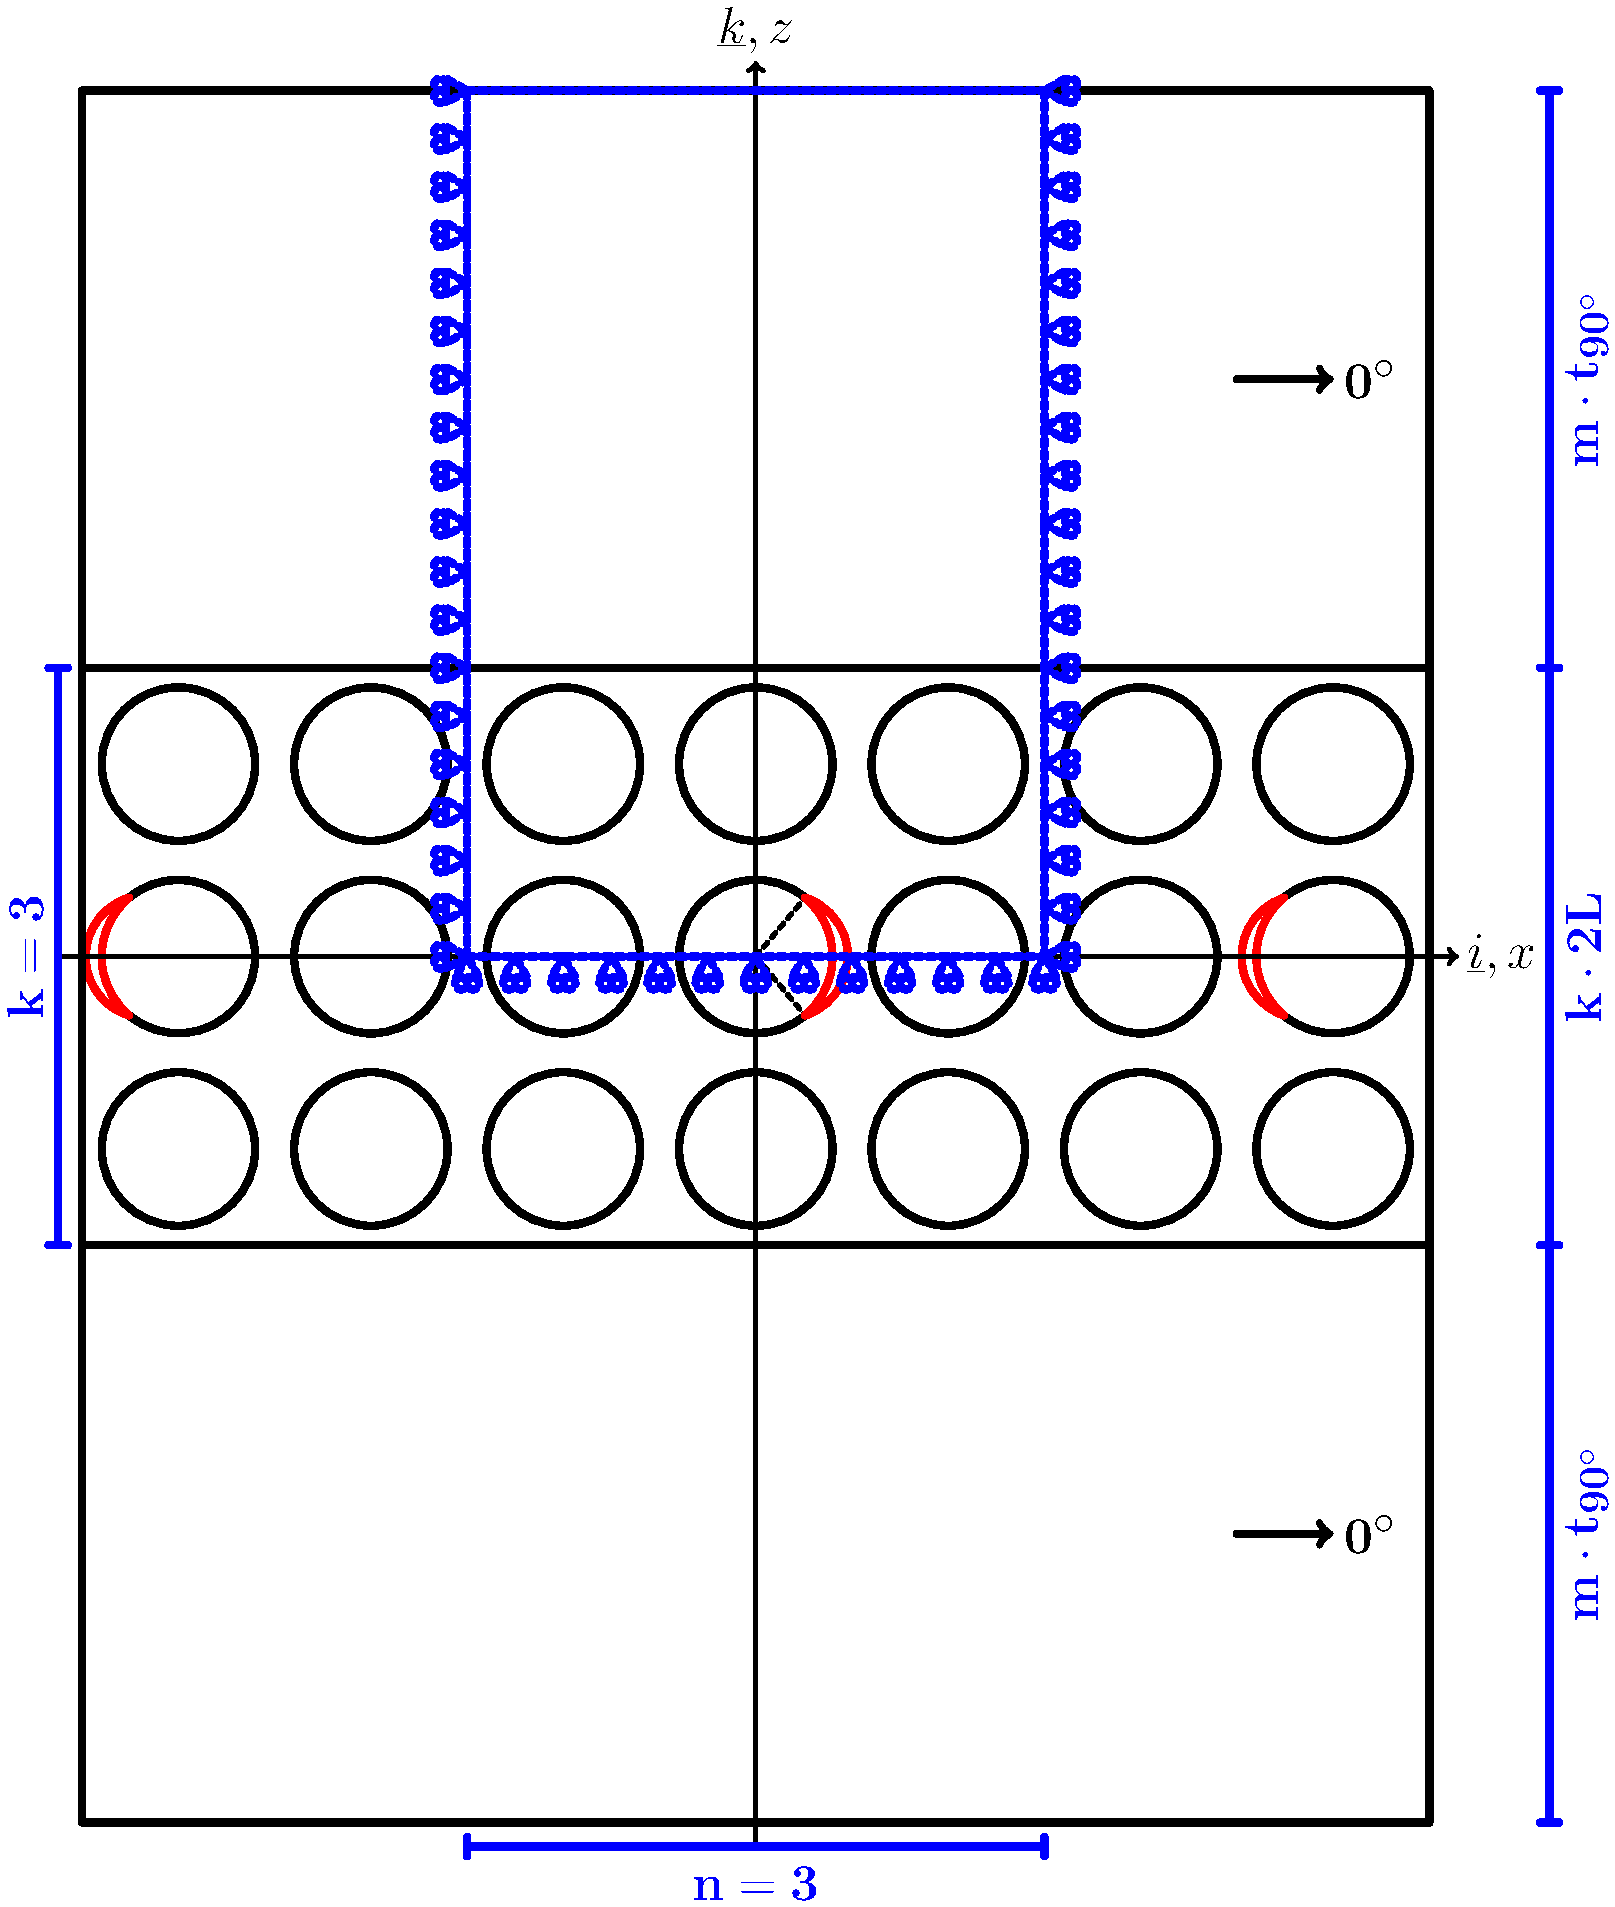
\includegraphics[width=\textwidth]{ThickPly.pdf}
   %    \caption{Mutiple rows of fibers with a debond appearing every $n$ fibers within the central row: model $n\times k-free$ ($n=3$ and $k=3$ in the figure).}\label{subfig:thickply}
\caption{Models of $\left[0_{m\cdot2l}^{\circ},90_{l}^{\circ}\right]_{S}$ laminates with a $90^{\circ}$ layer of variable thickness, determined by the number $k$ of ``rows'' of fibers along the vertical direction.  Debonds are repeating at different distances along the horizontal direction, measured in terms of the number $n-1$ of fully bonded fibers appearing between two consecutive debonds.}\label{fig:laminateModelsB}
\end{figure}

By increasing the number $n$ of fibers in the horizontal direction in the RUC, decreasing levels of damage (debonds spaced further apart and the interaction between debonds becomes less important) are considered to be present in the laminate. By increasing the number $k$ of fiber rows, the thickness of the $90^{\circ}$ layer is increased and the effect of the relative proximity of the inter-ply $0^{\circ}/90^{\circ}$ interface can thus be studied. Finally, by increasing the factor $m$, the thickness of the $0^{\circ}$ layers is increased for a given thickness of the $90^{\circ}$, which allows the investigation of the laminate thickness effect for a given ply thickness~\cite{Frossard2016}.

%% 2.3 Finite Element (FE) discretization

\subsection{Finite Element (FE) discretization}

The RUCs are discretized and solved with the Finite Element Method (FEM) using the commercial FEM package Abaqus~\cite{abq12}. The length $l$ and height $h$ of the model are determined by the number of fibers $n$ in the horizontal direction, the number of fiber rows $k$ across the thickness and the thickness ratio $i$ (see Sec.~\ref{subsec:rve}) according to Eq.~\ref{eq:lengthheight}:

\begin{equation}\label{eq:lengthheight}
l=2nL\qquad h=\left(1+2i\right)kL.
\end{equation}

In Eq.~\ref{eq:lengthheight}, $2L$ is the length of a one-fiber unit (see Fig.~\ref{fig:modelschem}), which in turn is as a function of the fiber volume fraction $V_{f}$ and the fiber radius according to

\begin{equation}\label{eq:LVf}
L=\frac{R_{f}}{2}\sqrt{\frac{\pi}{V_{f}}}.
\end{equation}

Each fiber in the model has the same radius $R_{f}$, equal to $1\ \mu m$. This specific value has no physical meaning per se and it has been selected for simplicity. It is useful to observe that, in a linear elastic solution as the one described in the present article, the ERR is proportional to the geometrical dimensions of the model and thus re-evaluation of the ERR for fibers of any size requires just a multiplication. Furthermore, the local and global $V_{f}$ are everywhere equal thanks to the relationships in Eqs.~\ref{eq:lengthheight} and~\ref{eq:LVf}.

\begin{figure}[!h]
\centering
        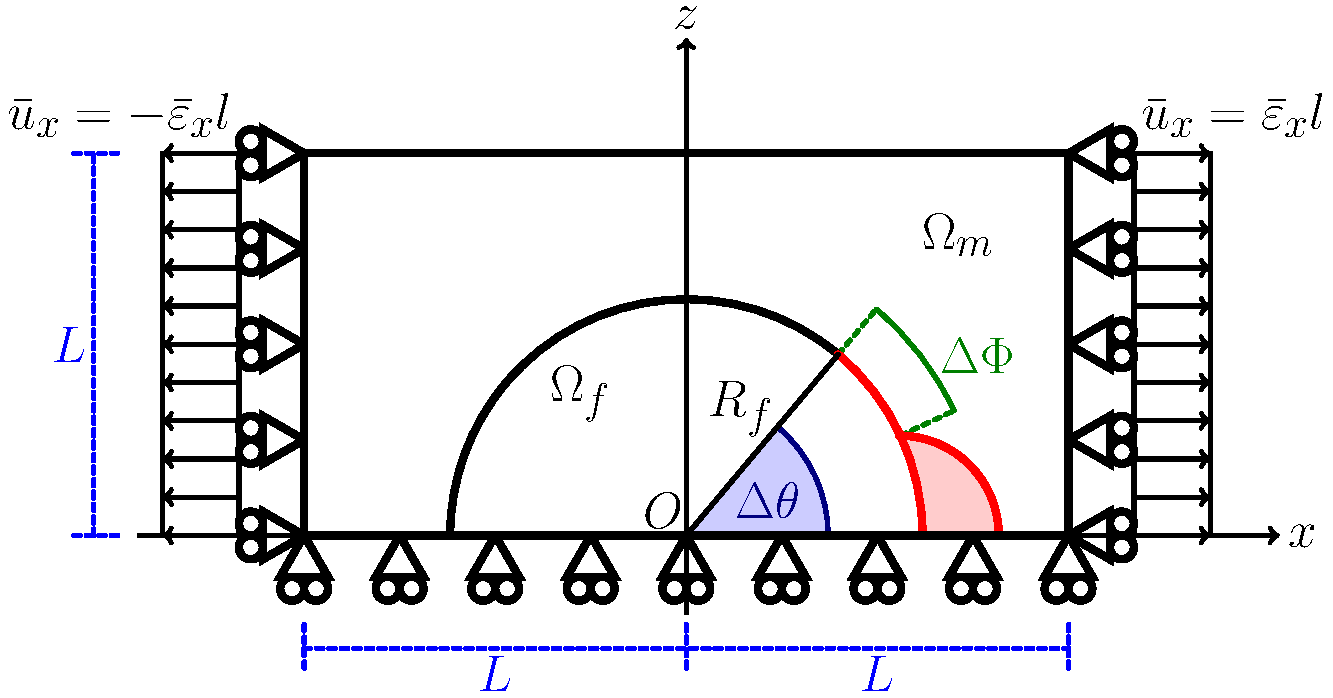
\includegraphics[width=\textwidth]{RUC.pdf}
\caption{Schematic of the model with its main parameters.}\label{fig:modelschem}
\end{figure}

The debond appears symmetrically with respect to the $x$ axis (see Fig.~\ref{fig:modelschem}) and we characterize it with the angular size $\Delta\theta$ (the full debond size is thus $2\Delta\theta$). In the case of large debond sizes ($\geq 60^{\circ}-80^{\circ}$), a region of size $\Delta\Phi$ to be determined by the solution itself appears at the crack tip. In this region, called the \emph{contact zone}, the crack faces are in contact and slide on each other. Due to existence of the contact zone, frictionless contact is considered between the two crack faces to avoid interpenetration and allow free sliding. Symmetry with respect to the $x$ axis is applied on the lower boundary. The upper boundary is free, except for the model $1\times 1-H+V$ which requires on the upper side kinematic coupling of vertical displacements and applied linearly distributed horizontal displacements. Kinematic coupling on the $x$-displacement is applied along the left and right boundaries of the model in the form of a constant $x$-displacement $\pm\bar{\varepsilon}_{x} l$, corresponding to transverse strain $\bar{\varepsilon}_{x}$ equal to $1\%$.

\begin{table}[!htbp]
 \centering
 \caption{Summary of mechanical properties of fiber, matrix and UD layer. $E$ stands for Young's modulus, $\mu$ for shear modulus and $\nu$ for Poisson's ratio. Indexes $L$ and $T$ stand respectively for \emph{longitudinal} and \emph{transverse}.}
 \begin{tabular}{ccccccc}
\textbf{Material} & \textbf{$V_{f}\left[\%\right]$}\  & \textbf{$E_{L}\left[GPa\right]$}\ & \textbf{$E_{T}\left[GPa\right]$}\  & \textbf{$\mu_{LT}\left[GPa\right]$} &\textbf{$\nu_{LT}\left[-\right]$} & \textbf{$\nu_{TT}\left[-\right]$} \\
\midrule
Glass fiber &-   & 70.0 & 70.0  & 29.2 & 0.2  & 0.2\\
Epoxy    &-& 3.5 & 3.5   & 1.25 &  0.4& 0.4\\
UD&60.0&43.442&13.714& 4.315& 0.273&0.465\\
\end{tabular}
\label{tab:phaseprop}
\end{table}

The FEM model is discretized using second order, 2D, plane strain triangular (CPE6) and rectangular (CPE8) elements. In the crack tip neighborhood, a refined regular mesh of quadrilateral elements with almost unitary aspect ratio is needed to ensure a correct evaluation of the ERR. The angular size $\delta$ of an element in this refined region close to the crack tip is by design equal to $0.05^{\circ}$. The crack faces are modeled as element-based surfaces with a frictionless small-sliding contact pair interaction. The Mode I, Mode II and total Energy Release Rates (ERRs) (respectively $G_{I}$, $G_{II}$ and $G_{TOT}$) represent the main result of the numerical analysis. They are computed using the VCCT~\cite{Krueger2004} implemented in a custom Python routine and the total ERR is obtained from the J-integral~\cite{Rice1968} evaluation by means of the Abaqus built-in functionality. Glass fiber and epoxy are considered throughout this article, and it is assumed that their response always lies in the linear elastic domain. The effective UD properties are computed using Hashin's Concentric Cylinder Assembly model~\cite{Hashin1983} with the self-consistency scheme for the out-of-plane shear modulus of Christensen~\cite{Christensen1979}. The properties used are listed in Table~\ref{tab:phaseprop}. The model was validated with respect to BEM results of~\cite{Paris2007,Sandino2016}; considerations about the order of accuracy can be found in~\cite{DiStasio2019}.

%%%%%%%%%%%%%%%%%%%%%%%%%%%%%%%%%%%%%%%%%%%%%%%%%%%%%%%%%%%%%%%%%%%
% 3. RESULTS AND DISCUSSION
%%%%%%%%%%%%%%%%%%%%%%%%%%%%%%%%%%%%%%%%%%%%%%%%%%%%%%%%%%%%%%%%%%%

\section{Results \& Discussion}

\subsection{Effect of the proximity of the $0^{\circ}/90^{\circ}$ interface and of the thickness of the $0^{\circ}$ layer on debond ERR}\label{subsec:thickness}

We first focus our attention on the model $1\times 1-m\cdot t_{90^{\circ}}$, which represents a particular case of the family $n\times 1-m\cdot t_{90^{\circ}}$. It corresponds to a cross-ply laminate in which the central $90^{\circ}$ ply is constituted by only one fiber row, in which each fiber possesses a debond appearing on alternating sides. The model thus represents an extreme idealization, in the sense that: first, the central $90^{\circ}$ layer is the thinniest that can be conceived; second, a very particular damage state is present for which every fiber is partially debonded from the sorrounding matrix. The first condition allows us to investigate the direct effect of the proximity of the $0^{\circ}/90^{\circ}$ interface on debond ERR. The second condition implies that we are analyzing the most severe damage state that can occur in the $90^{\circ}$ ply when considering debonds as the only mechanism of damage. As pointed out in a previous work~\cite{DiStasio2019}, the presence of fully bonded fibers close to the partially debonded one causes a magnification of the $x$-strain in the matrix region between the debonded fiber and the closest undamaged one. This increase in the value of the strain leads in turn to higher values of Energy Release Rate. Given that we are considering a $90^{\circ}$ ply with all fibers partially debonded, we are neglecting such magnification effect and focusing only on the presence of the $0^{\circ}/90^{\circ}$ interface and on the thickness of the $0^{\circ}$ layer, by considering the ratio $m=\frac{t_{0^{\circ}}}{t_{90^{\circ}}}$ of ply thicknessess as a free parameter. We will later analyze in Sec.~\ref{subsec:debonddebondinter} the effect of the combined presence of fully bonded fibers and the $0^{\circ}/90^{\circ}$ interface.

\begin{figure}[!h]
\centering
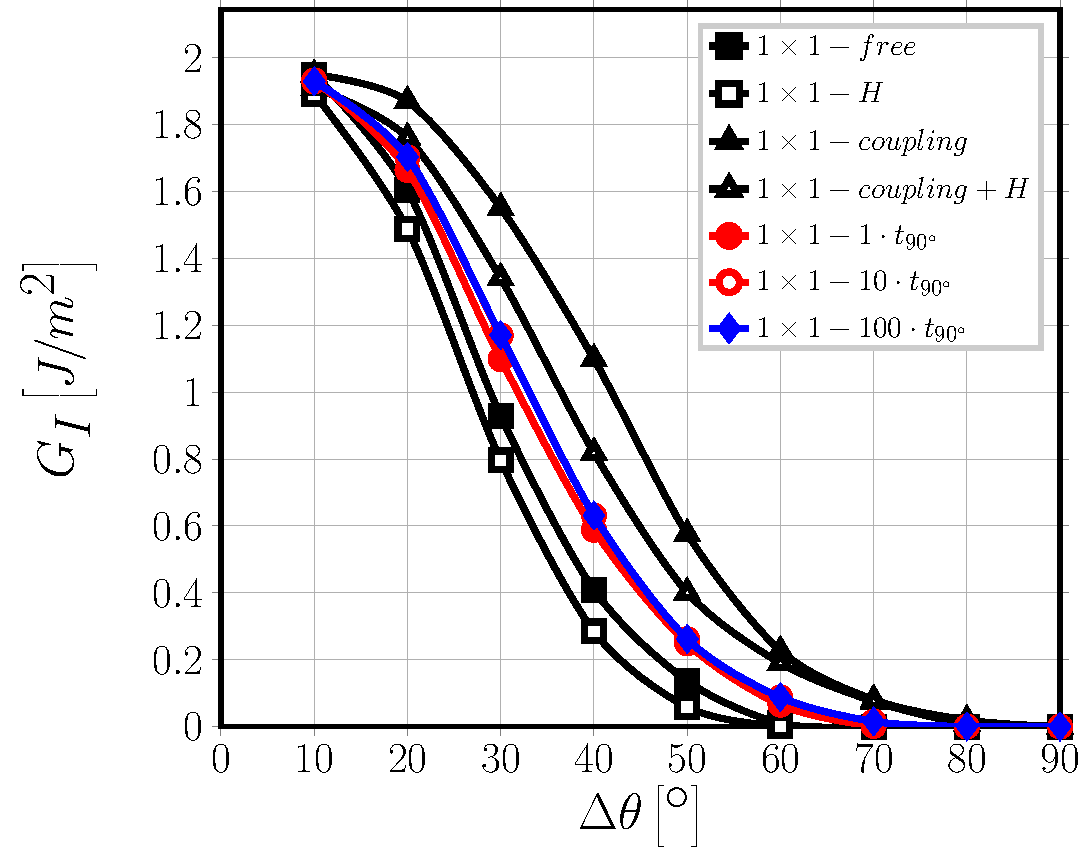
\includegraphics[width=\textwidth]{1x1-i-vf60-GI.pdf}
\caption{Effect of the proximity of the $0^{\circ}/90^{\circ}$ interface and of the thickness of the $0^{\circ}$ layer on Mode I ERR: models $1\times 1-free$, $1\times 1-coupling$, $1\times 1-H+V$ and $1\times 1-m\cdot t_{90^{\circ}}$. $V_{f}=60\%$, $\varepsilon_{x}=1\%$.}\label{fig:thicknessGI}
\end{figure}

In Figures~\ref{fig:thicknessGI} and~\ref{fig:thicknessGII} respectively the Mode I and Mode II ERR are shown for models $1\times 1-m\cdot t_{90^{\circ}}$ with $m=1,10,50,100$ and models $1\times 1-free$, $1\times 1-coupling$ and $1\times 1-H+V$. It is worth to remind us of the laminate RVE that correspond to these last three models: model $1\times 1-free$ represents a one-fiber-row UD composite with all the fibers partially debonded; model $1\times 1-coupling$ corresponds to a UD laminate with an infinite number of fiber rows and all the fibers partially debonded; model $1\times 1-H+V$ represents a cross-ply laminate with one-fiber-row central $90^{\circ}$ ply and the $0^{\circ}$ ply replaced by boundary conditions at the interface not allowing interface bending and with an applied uniform strain not affected by fibers and debonds in the $90^{\circ}$ ply. Observing Figure~\ref{fig:thicknessGI}, it is possible to notice that the values of $G_{I}$ for the $1\times 1-free$ and the $1\times 1-coupling$ model represent respectively a lower and an upper bound for all the other RVEs. The $1\times 1-H+V$ model is as well an upper bound for the $1\times 1-m\cdot t_{90^{\circ}}$ RVEs; however its values of $G_{I}$ are lower than those of the $1\times 1-coupling$ model due to the applied uniform $x$-strain at the interface, which prevents the crack to open as much as in the $1\times 1-coupling$ case. The same observation holds for the size of the debond at contact zone onset, i.e. when $G_{I}=0$: the lower bound is provided by the $1\times 1-free$ model ($\Delta\theta\sim60^{\circ}$), while the contact zone onset for models $1\times 1-coupling$ and $1\times 1-H+V$ represents the upper bound ($\sim80^{\circ}$). All $1\times 1-m\cdot t_{90^{\circ}}$ RVEs lie in between these two bounds for any thickness of the $0^{\circ}$ ply, with contact zone onset occurring at a debond size of $\sim70^{\circ}$.

%the presence of the $0^{\circ}/90^{\circ}$ $0^{\circ}/90^{\circ}$ interface translates into a modest increase in the value of $G_{I}$ with respect to the free surface. For every value of the thickness, however, the values of $G_{I}$ are lower than those computed with the $1\times 1-coupling$ and $1\times 1-H+V$ models. A more significant effect can be observed in relation to contact zone onset, which is delayed from $\Delta\theta=60^{\circ}$ in the presence of a free surface to $70^{\circ}$ in the presence of a homogenized $0^{\circ}$ layer. The maximum delay is however reached with the models with equivalent boundary conditions ($1\times 1-coupling$ and $1\times 1-H+V$), for which the contact zone onset happens at $\Delta\theta=80^{\circ}$. No effect of the thickness of the $0^{\circ}$ layer on Mode I ERR can be observed.

\begin{figure}[!h]
\centering
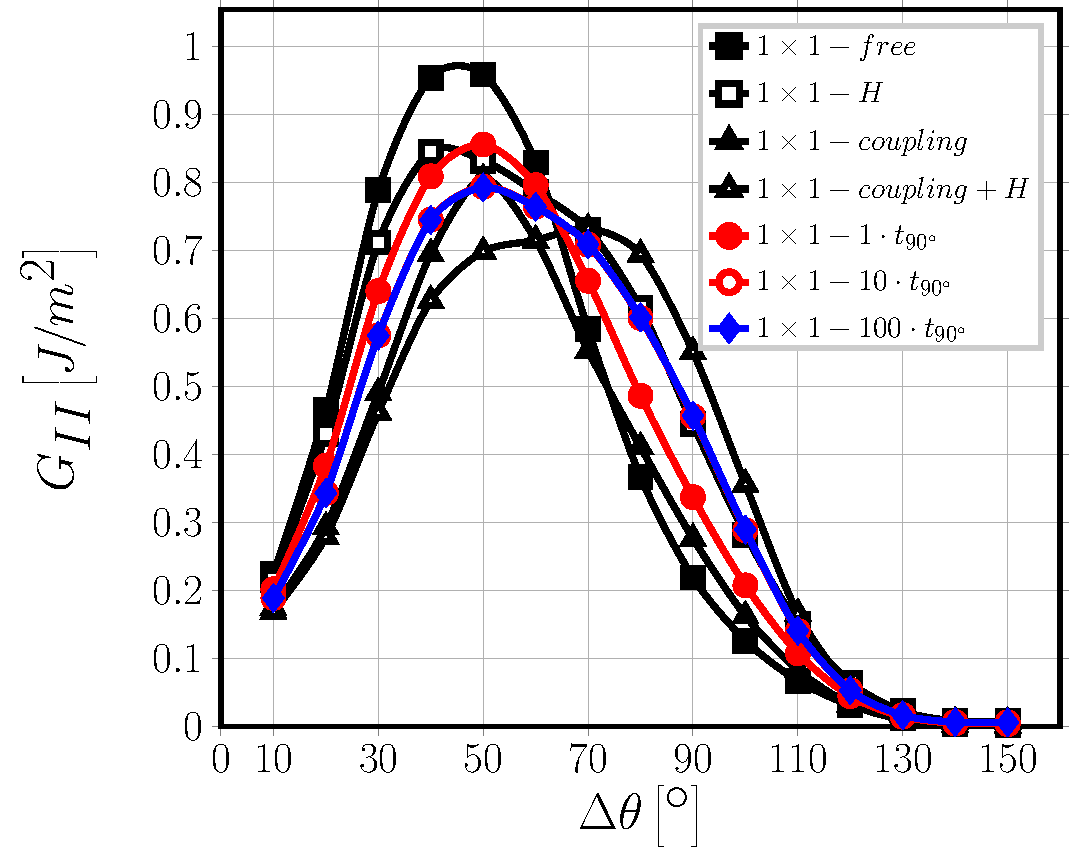
\includegraphics[width=\textwidth]{1x1-i-vf60-GII.pdf}
\caption{Effect of the proximity of the $0^{\circ}/90^{\circ}$ interface and of the thickness of the $0^{\circ}$ layer on Mode II ERR: models $1\times 1-free$, $1\times 1-coupling$, $1\times 1-H+V$ and $1\times 1-m\cdot t_{90^{\circ}}$. $V_{f}=60\%$, $\varepsilon_{x}=1\%$.}\label{fig:thicknessGII}
\end{figure}

For Mode II (see Fig.~\ref{fig:thicknessGII}), the ERR for the cases with a $0^{\circ}$ layer of finite thickness always lies between the values provided by the $1\times 1-free$ and $1\times 1-H+V$ model: for open debonds ($\Delta\theta<60^{\circ}-70^{\circ}$), when $G_{I}\neq0$ and there is no contact zone, $1\times 1-free$ provides the upper bound while $1\times 1-H+V$ the lower bound; for close debonds ($\Delta\theta>60^{\circ}-70^{\circ}$), when $G_{I}=0$ and a contact zone is present, the situation is reversed. An effect of the thickness of the $0^{\circ}$ layer on Mode II ERR can be noticed in Fig.~\ref{fig:thicknessGII} when the ratio $m=\frac{t_{0^{\circ}}}{t_{90^{\circ}}}$ is increased from $1$ to $10$. The change between the two follows the same pattern described previously: when the thickness of the $0^{\circ}$ ply is increased, Mode II decreases for open debonds and increases for closed debonds, in line with the bound switch.\\
These results help to shed light on the effect of the $0^{\circ}/90^{\circ}$ interface on debond ERR. The presence of the stiff homogenized $0^{\circ}$ layer causes the matrix placed relatively far from the fiber (close to the interface) to contract much less than it would do in the presence of a free surface due to its relatively high Poisson's ratio. Furthermore, the presence of the $0^{\circ}/90^{\circ}$ interface induces a more homogeneous $x$-displacement field all over the matrix domain. This causes a concurrent increase of $G_{I}$ and decrease of $G_{II}$ for small debonds, where the crack opening displacement component at the crack tip (responsible for Mode I) is mostly due to the global $x$-displacement field (which increases in the presence of the $0^{\circ}/90^{\circ}$  interface) while the crack sliding displacement component at the crack tip (responsible for Mode II) is for small debonds linked to the global vertical displacement field due to Poisson's effect (which is lower in the presence of a $0^{\circ}$ layer instead of a free surface thanks to the stiffness of the former). This causes also the delay in the onset of the contact zone. For large debonds instead, after the onset of the contact zone, the situation reverses: the magnitude increase of the global $x$-displacement field leads to an increase in the crack sliding displacement component at the crack tip and thus in Mode II ERR. By comparing the results for Mode II of models $1\times 1-free$, $1\times 1-H+V$ and $1\times 1-m\cdot t_{90^{\circ}}$ with $m=1,10,50,100$ (Fig.~\ref{fig:thicknessGII}), it can be argued that the effect of the $0^{\circ}$ ply thickness is related to its local bending stiffness. In the presence a free surface, the matrix in the $90^{\circ}$ ply contracts significantly more than the fibers due to the mismatch in Poisson's ratios, thus leading to higher $y$-strains in the inter-fibers regions than above the fibers. This in turn results in a very curved surface, roughly following the fibers' curvature. In the presence of a $0^{\circ}$ layer, such deformation is prevented by its bending stiffness. A relatively thin $0^{\circ}$ layer ($\frac{t_{0^{\circ}}}{t_{90^{\circ}}}=1$) possesses a lower bending stiffness and thus matrix deformation is able to bend the interface, which translates into a $G_{II}$ profile closer to the $1\times 1-free$ model. For thicker $0^{\circ}$ layers, the increased bending stiffness prevents the curvature of the interface and Mode II ERR becomes closer to the $1\times 1-H+V$ model, in which the interface is forced to remain straight by the applied boundary conditions.

\subsection{Effect of the proximity of the $0^{\circ}/90^{\circ}$ interface on debond-debond interaction in a single fiber row $90^{\circ}$ ply}\label{subsec:debonddebondinter}

We turn now our attention to the model $n\times 1-1\cdot t_{90^{\circ}}$, which corresponds to a cross-ply laminate in which the central $90^{\circ}$ ply is constituted by only one fiber row where multiple partially debonded fibers are present, located at a distance of $n-1$ fully bonded fibers from each other, and debonds appear on alternating sides of consecutive damaged fibers (see Figure~\ref{fig:laminateModelsA}). This class of models allows to study the effect of the presence of the $0^{\circ}$ layer on debond-debond interaction and, particularly, crack shielding~\cite{Garcia2015,DiStasio2019}.

\begin{figure}[!h]
\centering
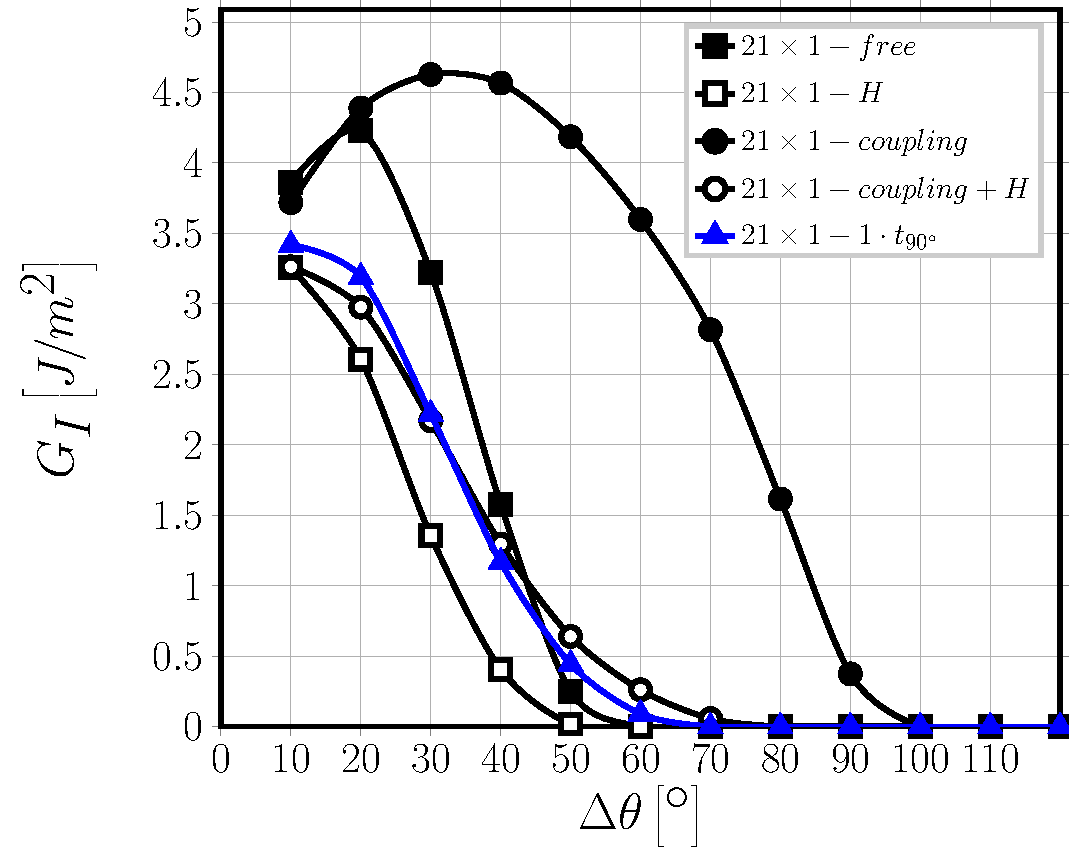
\includegraphics[width=\textwidth]{nx1-1-vf60-GI.pdf}
\caption{Effect of the presence of the $0^{\circ}$ layer on debond-debond interaction for Mode I ERR: models $n\times 1-free$ and $n\times 1-1\cdot t_{90^{\circ}}$. $V_{f}=60\%$, $\varepsilon_{x}=1\%$.}\label{fig:debonddebondGI}
\end{figure}

In the presence of a free surface, both Mode I and Mode II ERR increase rapidly when the number of fully bonded fibers placed between two consecutive partially debonded one is increased ($n\times 1-free$ models in Figures~\ref{fig:debonddebondGI} and ~\ref{fig:debonddebondGII}). The presence of fully bonded fibers causes an increase in the local $x$-strain in the debond neighborhood, which leads to greater crack opening and sliding displacements and thus higher ERR (strain magnification~\cite{DiStasio2019}). The same mechanism can be described from the opposite point of view: increasing the number of debonds present in the $90^{\circ}$ ply reduces the stress concentration in the inter-fibers regions and thus results in lower values of the ERR (crack shielding~\cite{Garcia2015,DiStasio2019}). From Figures~\ref{fig:debonddebondGI} and ~\ref{fig:debonddebondGII} it seems apparent that the strain magnification effect is present in cross-ply laminates as well, albeit strongly reduced by the presence of the $0^{\circ}/90^{\circ}$ interface. This effect is less evident when debonds are close to each other ($1\times 1-1\cdot t_{90^{\circ}}$ and $3\times 1-1\cdot t_{90^{\circ}}$), i.e. in the case of more severe damage states.

\begin{figure}[!h]
\centering
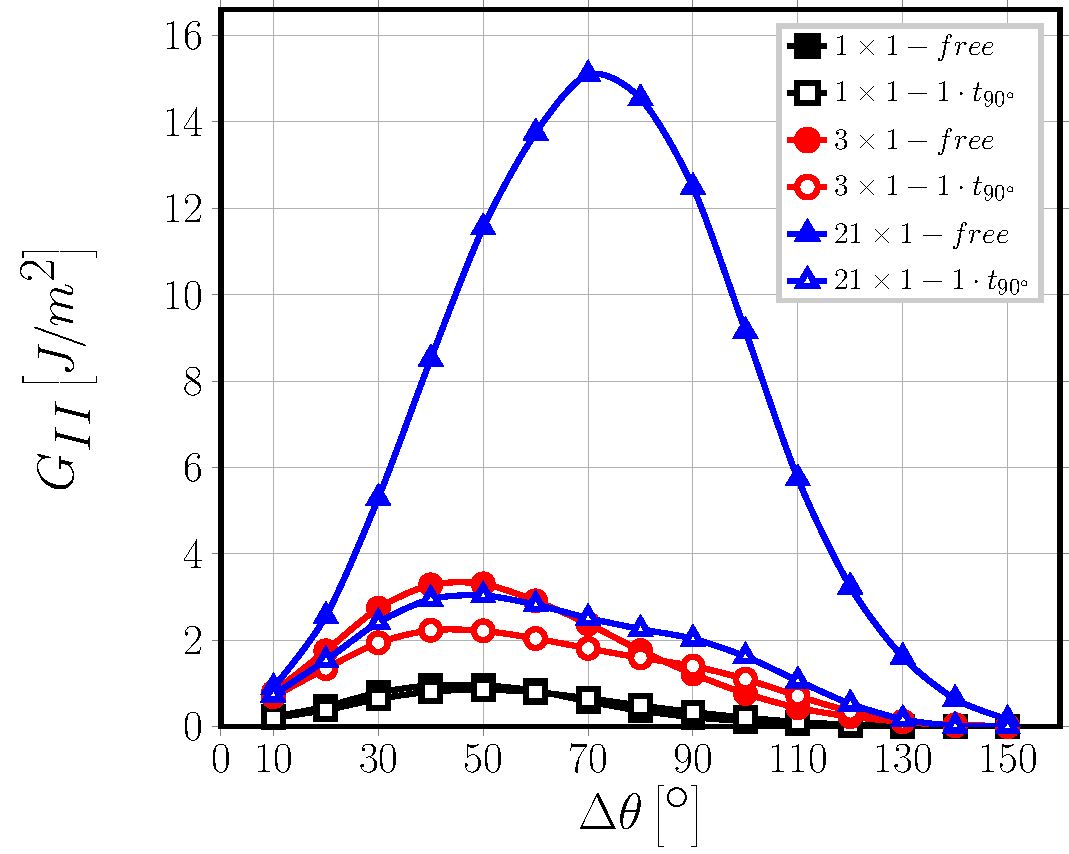
\includegraphics[width=\textwidth]{nx1-1-vf60-GII.pdf}
\caption{Effect of the presence of the $0^{\circ}$ layer on debond-debond interaction for Mode II ERR: models $n\times 1-free$ and $n\times 1-1\cdot t_{90^{\circ}}$. $V_{f}=60\%$, $\varepsilon_{x}=1\%$.}\label{fig:debonddebondGII}
\end{figure}

\subsection{Effect of the presence of fiber rows with no damage on the debond-$0^{\circ}/90^{\circ}$ $0^{\circ}/90^{\circ}$ interface interaction}

After having investigated the effect of the proximity of the $0^{\circ}/90^{\circ}$ interface and of the thickness of the $0^{\circ}$ layer on debond ERR and on debond-debond interaction, we address in this section the effect of the presence of fiber rows with only fully bonded fibers inside on the interaction between debonds and the $0^{\circ}/90^{\circ}$ interface. In other words, we are separating the debond from the interface by inserting rows of fully bonded fibers in between, thus increasing the distance to the interface. To this end, we study the models $1\times k-1\cdot t_{90^{\circ}}$, which represent a cross-ply laminate with the central $90^{\circ}$ ply made of $k$ fiber rows and where all the fibers in the central row are partially debonded. The absence of fully bonded fibers in the central row prevents the occurrence of strain magnification or crack shielding (see Sec.~\ref{subsec:debonddebondinter}), thus allowing to focus on the effect of the distance of the $0^{\circ}/90^{\circ}$ interface (measured in terms of rows of fully bonded fibers).

\begin{figure}[!h]
\centering
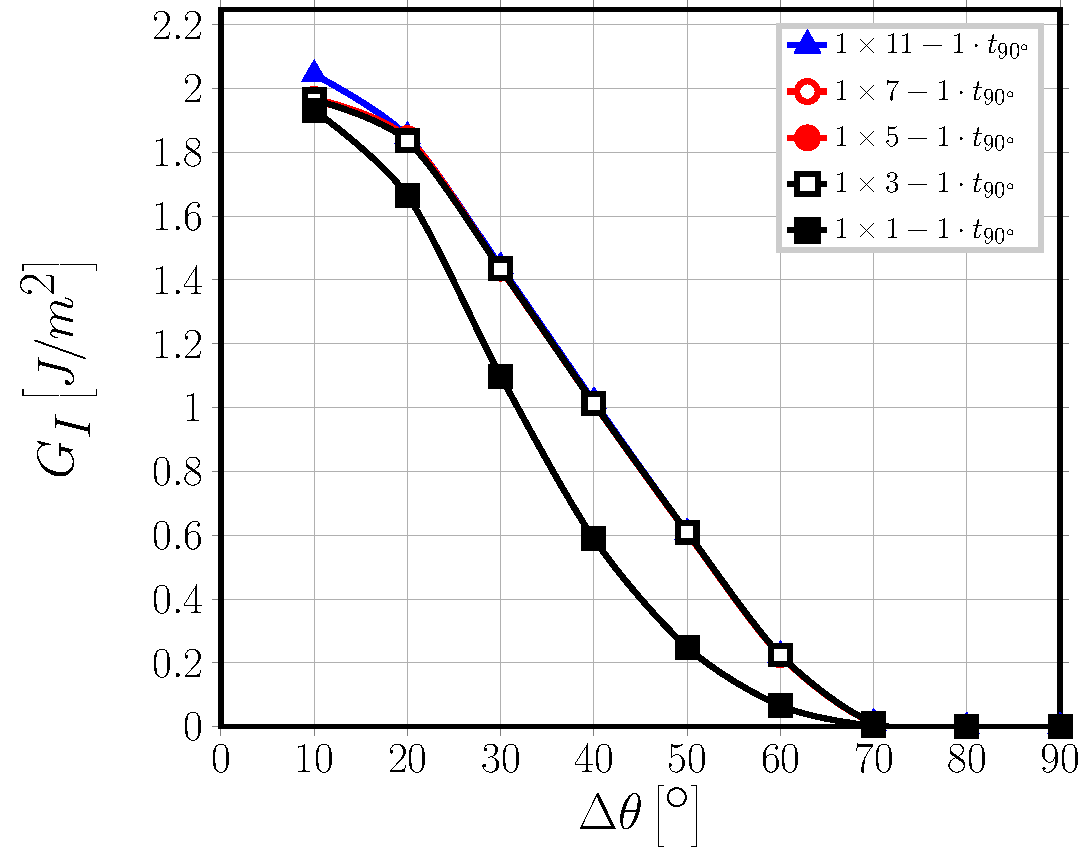
\includegraphics[width=\textwidth]{1xk-1-vf60-GI.pdf}
\caption{Effect of the presence of undamaged fiber rows in the $90^{\circ}$ layer on debond-$0^{\circ}/90^{\circ}$ interface interaction for Mode I ERR: models $1\times k-free$ and $1\times k-1\cdot t_{90^{\circ}}$. $V_{f}=60\%$, $\varepsilon_{x}=1\%$.}\label{fig:1kGI}
\end{figure}

Figures~\ref{fig:1kGI} and~\ref{fig:1kGII} thus show the effect on ERR of the presence of the $0^{\circ}$ ply in the case of non-interacting debonds (no strain magnification or crack shielding). If the distance between the $0^{\circ}/90^{\circ}$ interface and the debond is at least one fully bonded fiber, the presence of the $0^{\circ}$ ply does not influence debond ERR and no measurable difference can be observed between models $1\times k-free$ and $1\times k-1\cdot t_{90^{\circ}}$ for $k\geq1$.

\begin{figure}[!h]
\centering
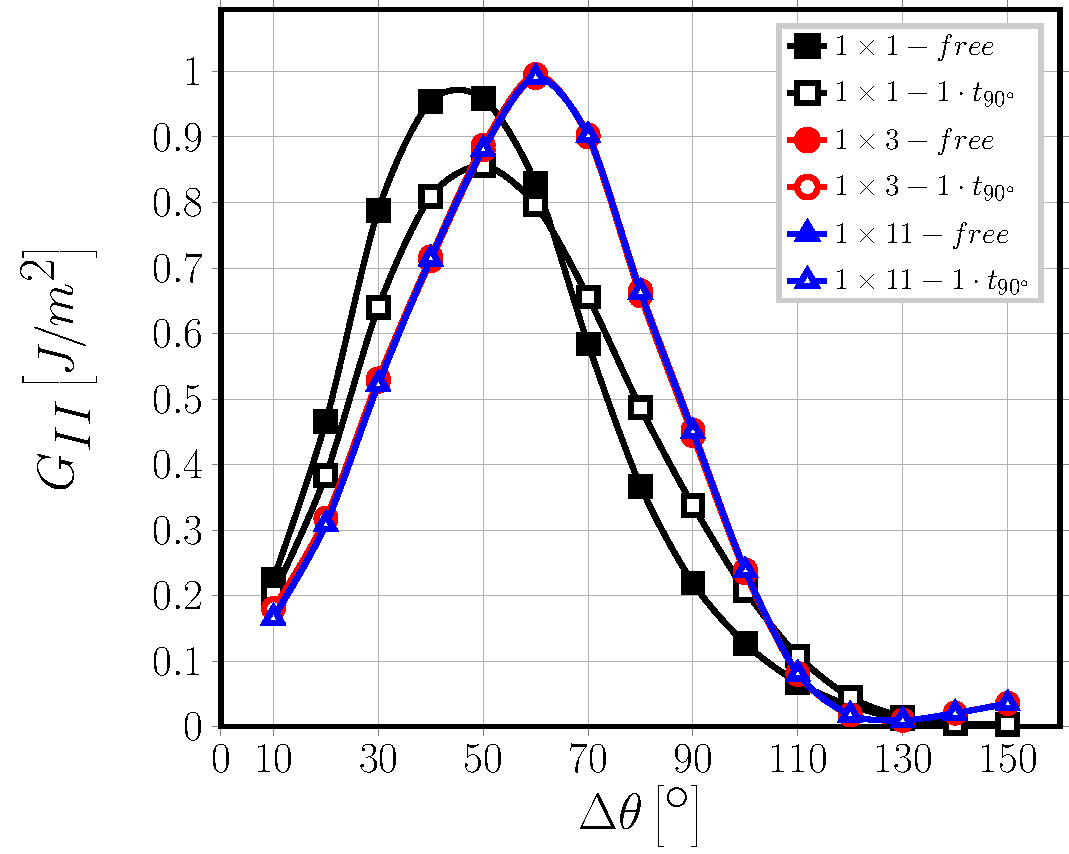
\includegraphics[width=\textwidth]{1xk-1-vf60-GII.pdf}
\caption{Effect of the presence of undamaged fiber rows in the $90^{\circ}$ layer on debond-$0^{\circ}/90^{\circ}$ interface interaction for Mode II ERR: models $1\times k-free$ and $1\times k-1\cdot t_{90^{\circ}}$. $V_{f}=60\%$, $\varepsilon_{x}=1\%$.}\label{fig:1kGII}
\end{figure}

\begin{figure}[!h]
\centering
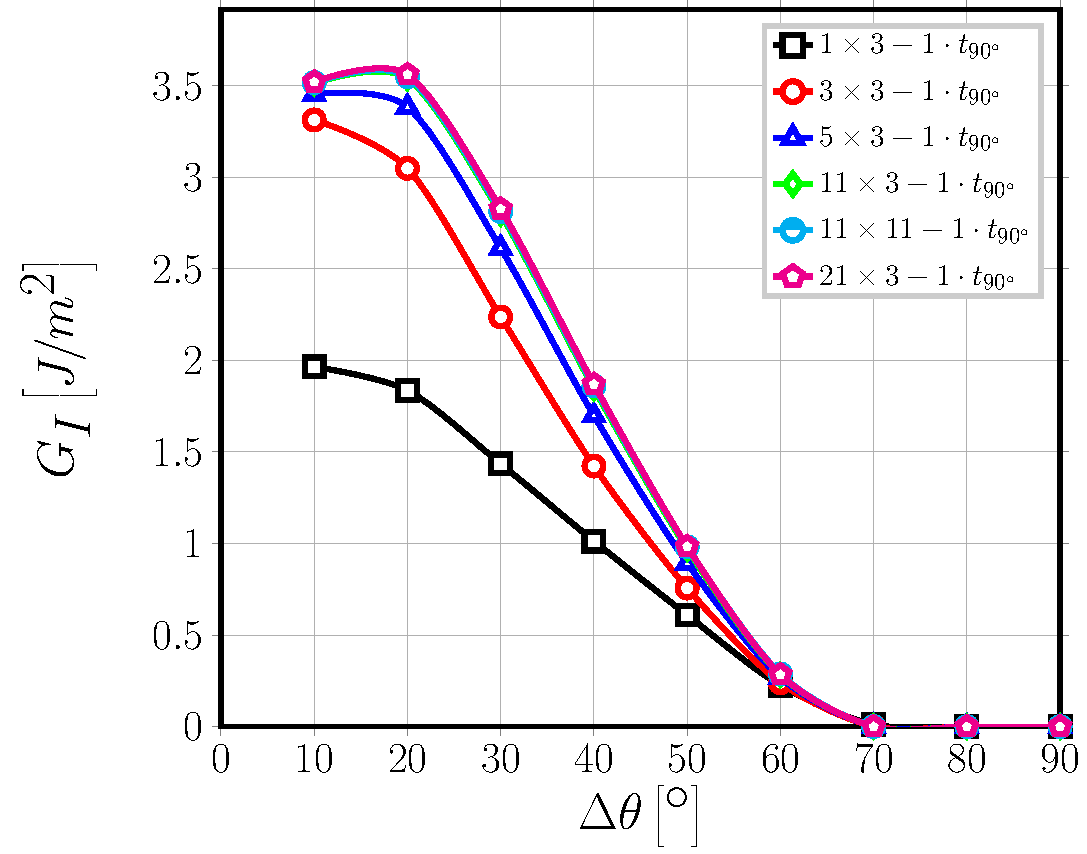
\includegraphics[width=\textwidth]{nxk-1-vf60-GI.pdf}
\caption{Effect of the presence of undamaged fiber rows in the $90^{\circ}$ layer on debond-$0^{\circ}/90^{\circ}$ interface interaction for Mode I ERR: models $n\times k-free$ and $n\times k-1\cdot t_{90^{\circ}}$. $V_{f}=60\%$, $\varepsilon_{x}=1\%$.}\label{fig:nkGI}
\end{figure}

However, the situation changes for interacting debonds, i.e. when fully bonded fibers are present between consecutive partially debonded fibers.

% Figures~\ref{fig:nkGI} and~\ref{fig:nkGII} the central fiber row of the $90^{\circ}$ layer possesses only partially debonded fibers, which represents an extreme damage state. It has been shown that the presence of fully bonded fibers causes a magnification of the $x$-strain in the debond neighborhood which leads to an increase in ERR both in one-fiber-row UD~\cite{DiStasio2019} and $90^{\circ}$ ply in cross-ply laminates (Sec.~\ref{subsec:debonddebondinter}). When rows of undamaged fibers are present above and below the fiber row containing the debonds, the presence of the $0^{\circ}/90^{\circ}$ $0^{\circ}/90^{\circ}$ interface has, with respect to the free surface case (corresponding to an extremely thin UD composite), no effect on $G_{I}$ and only a small effect on $G_{II}$, relevant only for thin $90^{\circ}$ plies (see Figures~\ref{fig:nkGI} and~\ref{fig:nkGII}). When present, this effect corresponds to a reduction in Mode II ERR, particularly for debonds further apart (in terms of number of fully bonded fibers between them).

\begin{figure}[!h]
\centering
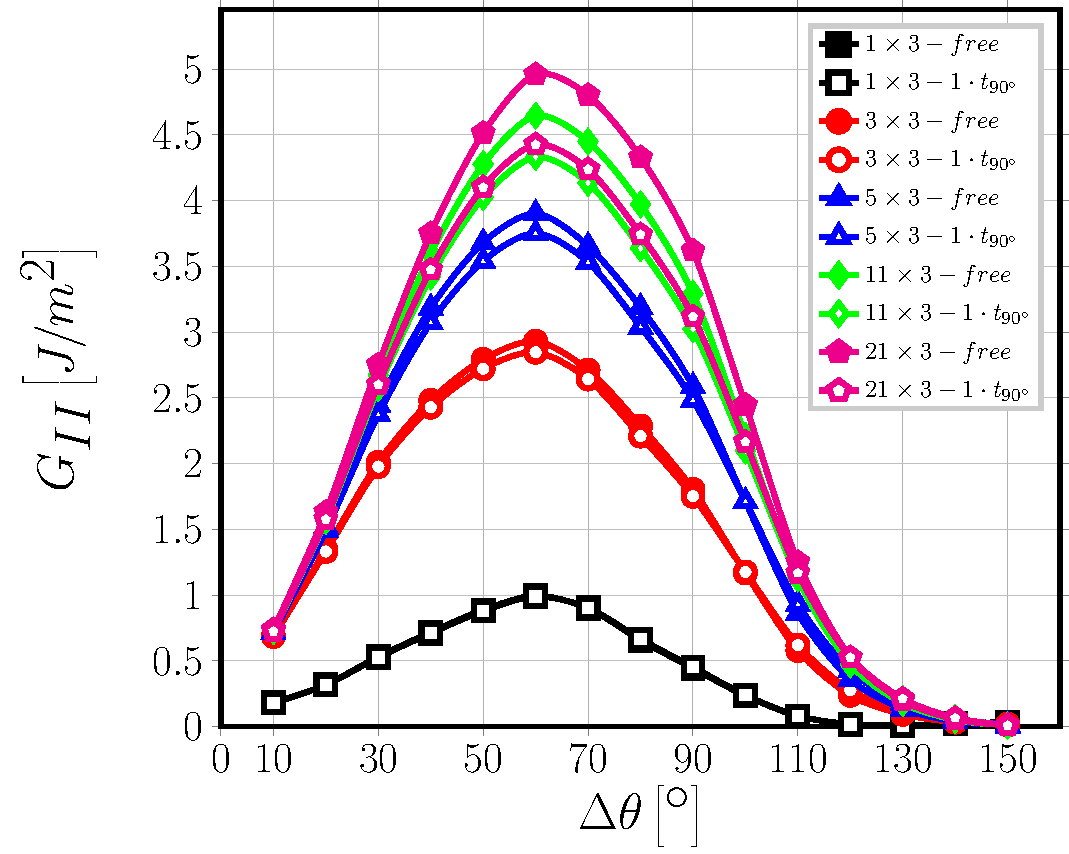
\includegraphics[width=\textwidth]{nxk-1-vf60-GII.pdf}
\caption{Effect of the presence of undamaged fiber rows in the $90^{\circ}$ layer on debond-$0^{\circ}/90^{\circ}$ interface interaction for Mode II ERR: models $n\times k-free$ and $n\times k-1\cdot t_{90^{\circ}}$. $V_{f}=60\%$, $\varepsilon_{x}=1\%$.}\label{fig:nkGII}
\end{figure}

In~\cite{Velasco2018, Paris2018}, the authors investigated the existence of scale effects (like the \emph{thin-ply effect}) in the context of the fiber-matrix interface crack using a single partially debonded fiber embedded in a homogenized $90^{\circ}$ ply bounded by homogenized $0^{\circ}$ layers. They observed the absence of any size effect. The results presented in this article confirm their observation and provide a micromechanical explanation (see Sec.○~\ref{subsec:thickness}). We have also shown that extremely thin $90^{\circ}$ plies ($1-5$ fibers across the thickness) do on the other hand present a magnification effect when fully bonded fibers appear between consecutive aligned debonds. The effect becomes stronger with thinner $90^{\circ}$ layers. The only effect of the $0^{\circ}$ ply is to reduce the magnification of ERR, which nonetheless takes place. However, this mechanism is not typical of cross-ply laminates, but it can be observed in UD composites as well~\cite{DiStasio2019}. It provides a possible mechanical description of the observations presented in~\cite{Saito2012}: in very thin $90^{\circ}$ plies debonds appear at lower strains because the magnification effect is stronger. As more debonds are created, their interaction (crack shielding) causes a reduction in ERR which disfavors debond growth.

%%%%%%%%%%%%%%%%%%%%%%%%%%%%%%%%%%%%%%%%%%%%%%%%%%%%%%%%%%%%%%%%%%%
% 4. CONCLUSIONS AND OUTLOOK
%%%%%%%%%%%%%%%%%%%%%%%%%%%%%%%%%%%%%%%%%%%%%%%%%%%%%%%%%%%%%%%%%%%

\section{Conclusions \& Outlook}

Different models of Repeating Unit Cell, representing different representative cross-ply laminates, have been studied in order to study the effect of the presence of the $0^{\circ}/90^{\circ}$ $0^{\circ}/90^{\circ}$ interface and of the thickness of the $0^{\circ}$ ply on debond Energy Release Rate and on crack shielding. It has been found that the presence of the $0^{\circ}$ ply causes only a reduction in ERR, especially in Mode II. However, the strain magnification effect due to the presence of fully bonded fibers between two consecutive debonds follows the same pattern previously identified for UD composites. Furthermore, the influence of the $0^{\circ}$ layer is strongly mitigated by the presence of rows of undamaged fibers. Already the presence of 1 row between respectively the upper and lower $0^{\circ}$ layer and the central fiber row with partially debonded fibers causes the computed Mode I and Mode II ERR to adhere closely to the results for a UD composite with the same geometrical configuration and damage state. The results presented provide an important insight: it appears that the behavior of the fiber/matrix interface crack is affected strongly only by very close perturbation of the elastic fields. \emph{Thin} and \emph{ultra-thin} plies present a peculiar behavior in terms of debond growth because their reduced thickness brings the $0^{\circ}/90^{\circ}$ $0^{\circ}/90^{\circ}$ interface close enough for the debonds to feel the perturbation in the elastic fields. Otherwise, it seems that no difference can be found in the mechanism of debond growth between a UD composite and a cross-ply laminate.

%%%%%%%%%%%%%%%%%%%%%%%%%%%%%%%%%%%%%%%%%%%%%%%%%%%%%%%%%%%%%%%%%%%
% ACKNOWLEDGEMENTS
%%%%%%%%%%%%%%%%%%%%%%%%%%%%%%%%%%%%%%%%%%%%%%%%%%%%%%%%%%%%%%%%%%%

\section*{Acknowledgements}

Luca Di Stasio gratefully acknowledges the support of the European School of Materials (EUSMAT) through the DocMASE Doctoral Programme and the European Commission through the Erasmus Mundus Programme.

%%%%%%%%%%%%%%%%%%%%%%%%%%%%%%%%%%%%%%%%%%%%%%%%%%%%%%%%%%%%%%%%%%%
% REFERENCES
%%%%%%%%%%%%%%%%%%%%%%%%%%%%%%%%%%%%%%%%%%%%%%%%%%%%%%%%%%%%%%%%%%%

\bibliography{refs}

\end{document}
